\documentclass{article}

\usepackage[utf8]{inputenc} 
\usepackage[russian]{babel} 
\usepackage{amsmath} 
\usepackage{hyperref} 
\usepackage{graphicx}
\usepackage{amssymb}
\newcommand{\numberset}[1]{\mathbb{#1}} 
\newcommand{\N}{\numberset{N}}
\newcommand{\Q}{\mathbb Q}
\newcommand{\R}{\mathbb R}
\newcommand{\Z}{\mathbb Z}
\usepackage[a4paper, total={6in, 8in}]{geometry}
\usepackage{color}
\usepackage{hyperref}
\hypersetup{
    colorlinks=true,
    linkcolor=blue,
    urlcolor=red,
    linktoc=all
}

\title{Матан коллок 12.11.2018}

\begin{document}
\maketitle 
\tableofcontents
\newpage
	\section{БИЛЕТ 1 -- Множества. Операции над ними. Свойства}
\begin{itemize}
\item \textbf{Множество} -- совокупность элементов, объектов, которые можно мыслить как единое целое.
\item Операции над множествами 
	\begin{enumerate}
	\item \textbf{Объединением} (суммой) множеств А и В называется множество $A \cup B$, элементы которого принадлежат хотя бы одному из этих множеств.
$$ A \cap B = \{ x : x \in A  \lor  x \in B \} $$
    \item \textbf{Пересечением} (произведением) множеств А и В называется множество $A \cap B$, элементы которого принадлежат как множеству А, так и множеству В.
$$ A \cup B = \{ x : x \in A \land x \in B \} $$
    \item \textbf{Разностью} множеств А и В называется множество $A \backslash B$, элементы которого принадлежат множеству А, но не принадлежат множеству В. 
    $$ A \backslash B = \{ x : x \in A \land x \notin B \} $$
    \item \textbf{Включение} множества B в множество А -- все элементы множества В принадлежат множеству А (\textit{нестрогое включение} –- возможен случай, что множество А состоит только из элементов множества В).
    $$ B \subset A = \{ x : x \in B \Rightarrow x \in A \} $$
    $ B \subset A \Rightarrow A \backslash B$ - дополнение множества В до А.
	\end{enumerate}
\item Свойства
\newline
\end{itemize}
\begin{center}
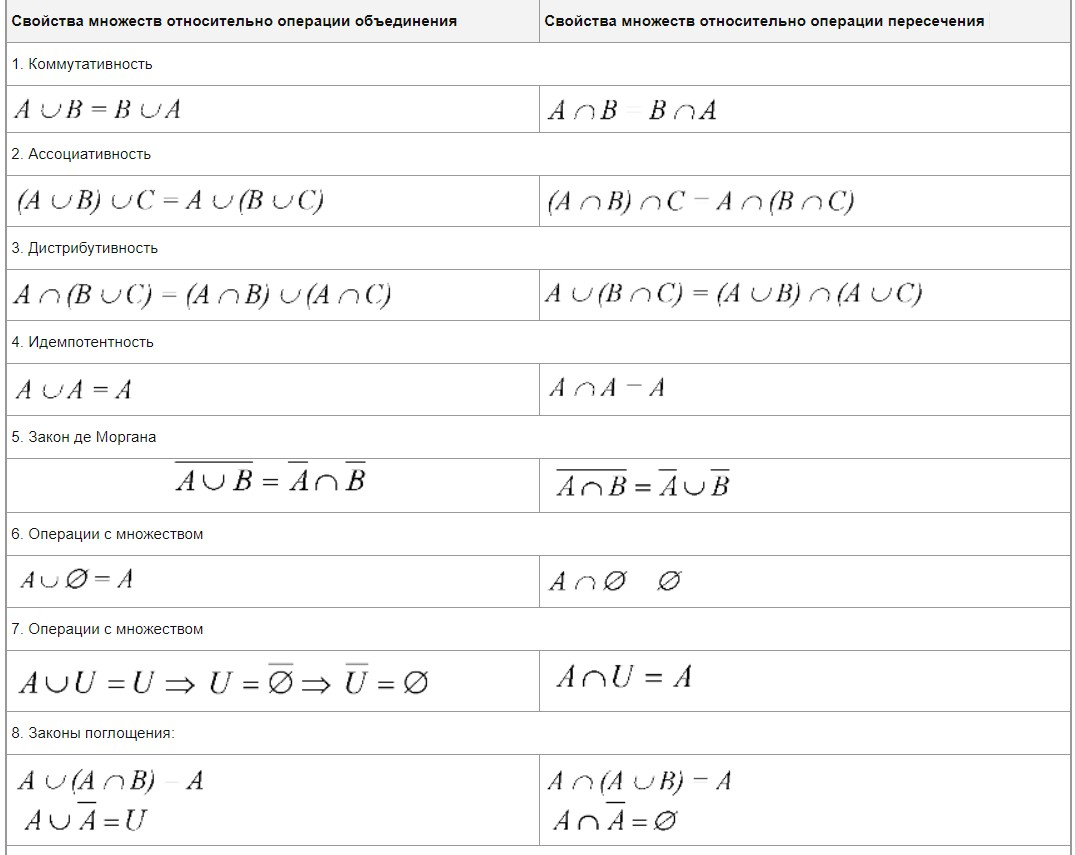
\includegraphics[scale=0.5]{1.jpg}
\end{center}
\newpage
\section{БИЛЕТ 2 -- Отображения. Функции}
$$f: X \to Y $$
\begin{itemize}
\item \textbf{Отображение} -- соответствие между элементами двух множеств, установленное по такому правилу, что каждому элементу одного множества ставится в соответствие некоторый элемент из другого множества. ($f: X \to Y $)
\item Функция \textbf{сюръективна}, если каждому элементу множества $Y$ может быть сопоставлен хотя бы один элемент множества $X$. То есть, функция $f$ сюръективна, если образ множества $X$ при отображении совпадает с множеством $Y$: $f(X)=Y$
\item Функция \textbf{инъективна}, если любым двум разным элементам из множества $X$ сопоставляются разные элементы из множества $Y$. Более формально, функция $f$ инъективна, если для любых двух элементов $x_{1}, x_{2} \in X$ таких, что $f(x_{1}) = f(x_{2})$, следует, что $x_{1}=x_{2}$. Другими словами, при инъекции не бывает так, чтобы два или больше разных элементов из множества $X$ отображались в один и тот же элемент из $Y$.
\item Функция \textbf{биективна}, если она одновременно сюръективна и инъективна.
\end{itemize}
\newpage
\section{БИЛЕТ 3 –- Аксиомы вещественных чисел}
\begin{enumerate}
\item Аксиомы сложения
\newline
$\forall a, b \in \R : a + b$
    \begin{enumerate}\alph*
    \item $a + b = b + a$
    \item $(a + b) + c = a + (b + c)$
    \item $\exists \;  0 : a + 0 = a$
    \item $\forall a \in \R \quad \exists -a : -a + a = 0$
    \end{enumerate}
\item Аксиомы умножения
\newline
$\forall a, b \in \R : a \cdot b$
    \begin{enumerate}\alph*
    \item $a \cdot b = b \cdot a$
    \item $a \cdot (b \cdot c) = (a \cdot b) \cdot c$
    \item $\exists \; 1 : a \cdot 1 = a$
    \item $\forall a \in \R, \;a \ne 0 \quad \exists \; a^{-1} : a^{-1} \cdot a = 1$
    \end{enumerate}
\item Дистрибутивность
\newline
$\forall a,b \in \R : (a + b) \cdot c = a \cdot c + b \cdot c$
\item Аксиомы сравнения
\newline
$\forall a,b,c \in \R$
    \begin{enumerate}\alph*
    \item $a > b, \: b > c \: \Rightarrow \: a > c$
    \item $a<b \: \Leftarrow \: a+c<b+c$
    \item $\forall c >0, \: a<b \: \Leftarrow \: a \cdot c < b \cdot c$
    \end{enumerate}
\item Непрерывность действительных чисел
\newline
$A \subset \R, \: B\subset \R$
\newline
$\forall a \in A, \:\forall b \in B, \: a<b \quad \exists \;\gamma \in \R: a<\gamma<b$
\end{enumerate}
\newpage
\section{БИЛЕТ 4 –- Неравенство Коши-Буняковского}
\begin{center}
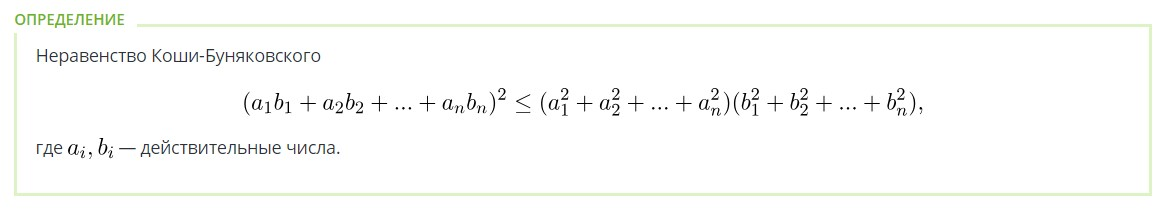
\includegraphics[scale=0.6]{2.jpg}
\end{center}
\textbf{Доказательство}:
\begin{center}
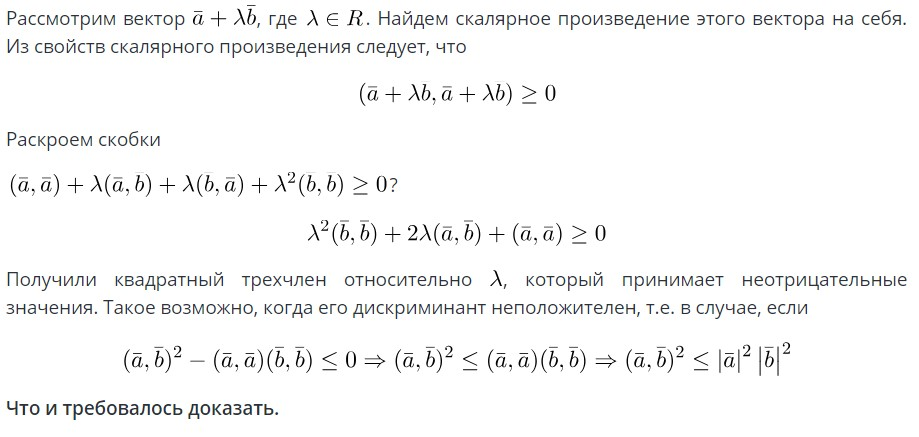
\includegraphics[scale=0.8]{3.jpg}
\end{center}
\newpage
\section{БИЛЕТ 5 –- Счётные множества. Два простейших свойства}
Множество X называется \textbf{счетным}, если оно равномощно* множеству натуральных чисел N.
Свойства
\begin{enumerate}
    \item Любое бесконечное множество содержит бесконечное счетное подмножество.
    \newline
    \newline
    \textbf{Доказательство}:
    \begin{itemize}
    \item Пусть $X$ -- бесконечное множество; тогда оно во всяком случае непусто, т. е. в нем существует по крайней мере один элемент, обозначим его через $x_{1}$. Поскольку множество $X$ бесконечно, то множество $X \backslash \{x_{1}\}$ также непусто, т. е. содержит по крайней мере один элемент, обозначим его $x_{2}$. Продолжая этот процесс, на $n$-м шаге получим элемент $x_{n}$. Поскольку $X$ - бесконечное множество, то множество $X \backslash \{x_{1}, x_{2}, ..., x_{n}\}$ непусто, т. е. содержит по крайней мере один элемент, обозначим его $x_{n+1}$ и т. д. Множество $\{x_{1}, x_{2}, ..., x_{n}, ...\}$ - искомое счетное подмножество множества $X$.
    \end{itemize}
    \item Любое бесконечное подмножество счетного множества счетно.
    \newline
    \newline
    \textbf{Доказательство}:
    \begin{itemize}
        \item Пусть $X$ -- счетное множество: $X = \{x_{1}, x_{2}, ..., x_{n}, ...\}$  и $Y$ включает $X$. Обозначим через $y_{1}$ элемент из $Y$, имеющий наименьший номер в $X$, через  $y_{2}$ -- элемент множества $Y$, имеющий следующий ближайший номер, и т. д. Поскольку каждый элемент множества $Y$ является некоторым элементом $x_{n}$ множества $X$ и, следовательно, имеет номер $n$, то через конечное число шагов (не больше, чем $n$) он получает некоторый номер $m$ и в множестве $Y$, т. е. будет обозначен $y_{m}$, причем, поскольку множество $Y$ бесконечно, этот процесс может быть продолжен неограниченно. Таким образом, все элементы множества $Y$ окажутся перенумерованными, что и означает счетность этого множества.
    \end{itemize}
    \end{enumerate}
* Два множества, между элементами которых можно установить взаимно однозначное соответствие (биекцию), называются \textit{равномощными}.
\newpage
\section{БИЛЕТ 6 –- Счётность множества рациональных чисел}
\textbf{ТЕОРЕМА}. Множество всех рациональных чисел счетно. 
\newline
\newline
\textbf{Доказательство}:
Расположим все рациональные числа в таблицу, содержащую бесконечное число строк и столбцов, следующим образом (см. таблицу):
    \newline
    \begin{center}
    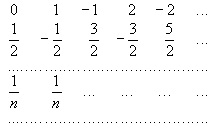
\includegraphics[scale=1.5]{4.jpg}
    \end{center}
     Здесь в $n$-ю строчку помещены рациональные числа, записываемые несократимыми рациональными дробями со знаменателем $n$ и упорядоченные по возрастанию их абсолютных величин, причем непосредственно за каждым положительным числом следует ему противоположное. Очевидно, что каждое рациональное число находится на каком-то месте в этой таблице.
     \newline
     \newline
     Занумеруем теперь элементы получившейся таблицы согласно следующей схеме, в которой в кружочках стоят номера соответствующих элементов, а стрелки указывают направление нумерации. В результате все рациональные числа оказываются занумерованными, т. е. множество $\Q$ рациональных чисел счетно.
     \newline
     \begin{center}
     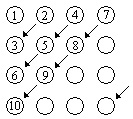
\includegraphics[scale=1.5]{6.jpg}
     \end{center}
\newpage
\section{БИЛЕТ 7 -- Несчётность отрезка}
Любой отрезок множества действительных чисел состоит из несчетного множества точек.
\newline
\newline
\textbf{Доказательство}:
\newline
\newline
Допустим противное: пусть точки некоторого отрезка $[\,a,b\,]$, $a$ принадлежит $\R$, $b$ принадлежит $\R$, $a < b$, можно занумеровать: $[\,a,b\,] = \{x_{1},x_{2}...,x_{n},...\}$. Выберем акой-либо отрезок $[\,a_{1},b_{1}\,]$ лежащий на $[\,a,b\,]$ и не содержащий точки $x_{1}$ (см рис.):
    \newline
    \newline
    \begin{center}
    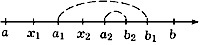
\includegraphics[scale=1.5]{5.jpg}
    \end{center}
    $$ x_{1} \notin [\,a_{1},b_{1}\,] \subset [\,a,b\,] $$
    Далее выберем отрезок $[\,a_{2},b_{2}\,]$, лежащий на $[\,a_{1},b_{1}\,]$ и не содержащий точки $x_{2}$, и т. д. Таким образом, если выбран отрезок $[\,a_{n},b_{n}\,]$, то выберем отрезок $[\,a_{n+1},b_{n+1}\,]$, лежащий на $[\,a_{n},b_{n}\,]$ и не содержащий точки $x_{n+1}$. Продолжая этот процесс, получим систему вложенных отрезков $[\,a_{n},b_{n}\,]$, $n = 1, 2, ...$, такую, что
    \begin{equation}
        \setcounter{equation}{1}
         x_{n} \notin [\,a_{n},b_{n}\,],\,n = 1, 2, ... 
    \end{equation}
     Следовательно, ни одна точка $x_{n}$ не принадлежит пересечению $[\,a_{n},b_{n}\,]$, но согласно принципу вложенных отрезков существует точка, обозначим ее $\xi$, принадлежащая всем отрезкам $[\,a_{n},b_{n}\,]$:
     \begin{equation}
         \xi \in [\,a_{n},b_{n}\,], \,n = 1, 2, ...,
     \end{equation} 
     а поэтому и отрезку $[\,a,b\,]$, ибо $[\,a_{n},b_{n}\,]$ включает $[\,a,b\,]$ при всех   $n = 1, 2, ...$ А так как все точки отрезка $[\,a,b\,]$ по предположению перенумерованы, то точка $\xi$ также должна иметь какой-то номер, т. е. существует такое натуральное число $X_{n_{0}}$, что $\xi = x_{n_{0}}$, и тогда согласно (2) получим:
     $$ x_{n_{0}} \in [\,a_{n},b_{n}\,], n = 1, 2, ... $$
     В частности, $ x_{n_{0}} \in [\,a_{n_{0}},b_{n_{0}}\,]$, а это противоречит условию (1). 
\newpage
\section{БИЛЕТ 8 -- Единственность предела и ограниченность сходящейся последовательности}
Точка $a$ (конечная или бесконечно удаленная) числовой прямой называется \textbf{пределом} некоторой числовой последовательности действительных чисел, если, какова бы ни была окрестность точки $a$, она содержит все члены рассматриваемой последовательности начиная с некоторого номера.
$$a=\lim_{n\to\infty} f(x)\Leftrightarrow \; \exists \: n_{\xi} \:\: \forall n>n_{\xi} : x_{n} \in U(a, \xi)$$
Если числовая последовательность имеет конечный предел, то она называется \textbf{сходящейся}.
$$\exists \: a \in \R \:\: \forall \xi > 0 \:\: \exists \: n_{\xi} \in \N \:\: \forall n > n_{\xi} : |x_{n} - a|<\xi$$
$$ a=\lim_{n\to\infty} x_{n} \Leftrightarrow \; \forall \xi > 0 \:\:\exists \: n_{\xi} \in\N \:\:\forall n>n_{\xi} : a-\xi<x_{n}<a+\xi $$
\paragraph{ЕДИНСТВЕННОСТЬ ПРЕДЕЛА.}
Последовательность точек расширенной числовой прямой может иметь на этой прямой только один предел.
\newline
\newline
\textbf{Доказательство} (методом от противного):
$$ \lim_{n\to\infty} x_{n}=a, \:\: \lim_{n\to\infty} x_{n}=b $$
Выберем непересекающиеся окрестности: $$\xi_{1} > 0, \xi_{2}>0 : U(a,\xi_{1}) \cap U(b,\xi_{2}) = \varnothing .$$
$$ \lim_{n\to\infty} x_{n}=a \Rightarrow \: \exists \: n_{1} \;\; \forall n>n_{1} : x_{n}\in U(a,\xi_{1}); $$
$$ \lim_{n\to\infty} x_{n}=b \Rightarrow \: \exists \: n_{2} \;\; \forall n>n_{1} : x_{n}\in U(b,\xi_{2}); $$
$$ n_{0}=max(n_{1},n_{2}):\forall n>n_{0}:x_{n}\in U(a,\xi_{1}) \land x_{n}\in U(b, \xi_{2}) \Rightarrow $$
$$ \Rightarrow \: x_{n}\in [\,U(a,\xi_{1})\cap U(b,\xi_{2})\,]\land [\,U(a,\xi_{1})\cap U(b,\xi_{2})\,] = \varnothing$$
Пришли к полной чепухе, значит, верно обратное.
\paragraph{ОГРАНИЧЕННОСТЬ ЧИСЛОВОЙ ПОСЛЕДОВАТЕЛЬНОСТИ.}
Если числовая последовательность имеет конечный предел, то она ограничена. 
\newline
\newline
\textbf{Доказательство}:
\newline
Пусть $$\lim_{n\to\infty} x_{n}=a,\xi=1,$$ тогда:
$$ \exists \: n_{0} \:\forall n>n_{0} : |x_{n}-a|<1. $$
$$ d=max(1,|x_{1}-a|,|x_{2}-a|,\ldots,|x_{n}-a|) \Rightarrow $$
$$ \Rightarrow\:\:|x_{n}-a|<d,\:\:a-d<x_{n}<a+d. $$
\newpage
\section{БИЛЕТ 9 -- Теорема о предельном переходе в неравенствах}
$$ x_{n},y_{n},a,b\in\R,\, \lim_{n\to\infty} x_{n}=a,\lim_{n\to\infty} y_{n}=b,\: a<b\:\Rightarrow  $$
$$ \Rightarrow\:\exists\:n_{0}\:\:\forall n>n_{0}:x_{n}<y_{n} $$
\textbf{Доказательство}:
\newline
\newline
Пусть $U(a)\cap V(b)=\varnothing$.
$$\forall x\in U \land y\in V,\: x<y$$
$$\exists \:n_{0}\:\forall n>n_{0}:x_{n}\in U,y_{n}\in V\:\Rightarrow$$
$$\Rightarrow\:\exists\:n_{0}\:\forall n>n_{0}:x_{n}<y_{n}$$
\newpage
\section{БИЛЕТ 10 -- Теорема о двух городовых}
$$x_{n},y_{n},z_{n}\in\R,x_{n}\leqslant y_{n}\leqslant z_{n} \:\land \:\lim_{n\to\infty} x_{n}=\lim_{n\to\infty} z_{n}=a\in\R \:\Rightarrow\:\lim_{n\to\infty}y_{n}=a$$
\textbf{Доказательство}:
\newline
\newline
Выберем произволньую окрестность точки $a$: $U(a)$.
$$\lim_{n\to\infty} x_{n}=a \Rightarrow \: \exists \: n_{1} \;\; \forall n>n_{1} : x_{n}\in U(a);$$
$$\lim_{n\to\infty} z_{n}=a \Rightarrow \: \exists \: n_{2} \;\; \forall n>n_{2} : z_{n}\in U(a);$$
$$ n_{0}=max(n_{1},n_{2}):\:x_{n}\in U(a)\land z_{n}\in U(a) \:\forall n>n_{0}\:\Rightarrow $$
$$ \Rightarrow\:y_{n}\in U(a)\:\forall n>n_{0}\:\Rightarrow\: \lim_{n\to\infty} y_{n}=a$$
\newpage
\section{БИЛЕТ 11 -- Бесконечно малая последовательность}
Бесконечная малая последовательность:
$$ \lim_{n\to\infty} a_{n} = 0 $$
\begin{itemize}
    \item Любая конечная линейная комбинация бесконечно малых является бесконечно малой.
    $$ \lim_{n\to\infty} \alpha_{n} = \lim_{n\to\infty} \beta_{n}=0\:\Rightarrow\:\lim_{n\to\infty} (\lambda\cdot \alpha_{n}+\lambda\cdot\beta_{n})=0 $$
    \textbf{Доказательство}:
    $$ c>|\lambda|+|\mu| $$
    $$ \exists\:n_{0}\:\forall n>n_{0}:|\alpha_{n}|<\frac{\xi}{c}, \:|\beta_{n}|<\frac{\xi}{c};$$
    $$ |\lambda\cdot\alpha_{n}+\mu\cdot\beta_{n}|\leqslant |\lambda|\cdot|\alpha_{n}|+|\mu|\cdot|\beta_{n}|<\frac{|\lambda|+|\mu|}{c}\cdot\xi<\xi $$
    \item Произведение бесконечно малой последовательности на ограниченную последовательность является бесконечно малой последовательностью.
    $$ \lim_{n\to\infty}\alpha_{n}=0,\qquad \exists\:b\:\forall n\in\N:|x_{n}|\leqslant b.$$
    $$ \forall n>n_{\xi}:|\alpha_{n}|<\frac{\xi}{b}, $$
    $$ |\alpha_{n}\cdot x_{n}|=|\alpha_{n}|\cdot|x_{n}|<\frac{\xi}{b}\cdot b=\xi $$
    \item Произведение конечного числа бесконечно малых последовательностей является бесконечно малой последовательностью.
    \item Предел обратной последовательности от бесконечно малой равен бесконечности.
    $$\lim_{n\to\infty}x_{n}=0\:\Leftrightarrow\:\lim_{n\to\infty}\frac{1}{x_{n}}=\infty$$
\end{itemize}
\newpage
\section{БИЛЕТ 12 -- Теорема об арифметичских свойствах предела}
\begin{enumerate}
    \item Добавление (?)
    $$ \lim_{n\to\infty} x_{n}=a\:\Leftrightarrow\:x_{n}=a+\alpha_{n},\, \{\alpha_{n}\}\to 0. $$
    \textbf{Доказательство}:
    $$ \alpha_{n}=|x_{n}-a|. $$ 
    $$ \lim_{n\to\infty}x_{n}=a\:\Leftrightarrow\:\forall\xi>0\:\:\exists\:n_{0}\:\forall n>n_{0}: $$
    $$ |x_{n}-a|<\xi\:\Leftrightarrow\:\lim_{n\to\infty}\alpha_{n}=0. $$
    \item Конечная линейная комбинация сходящихся последовательностей -- сходящаяся последовательность, и ее предел равен такой же линейной комбинации пределов данных последовательностей.
    $$\lim_{n\to\infty}(\lambda\cdot x_{n}+\mu\cdot y_{n})=\lambda\cdot\lim_{n\to\infty}x_{n}+\mu\cdot\lim_{n\to\infty}y_{n}. $$
    \textbf{Доказательство}:
    $$\lim_{n\to\infty}x_{n}=a\in\R,\,\lim_{n\to\infty}y_{n}=b\in\R;\:\lim_{n\to\infty}\alpha_{n}=\lim_{n\to\infty}\beta_{n}=0.$$
    $$ x_{n}=a+\alpha_{n},\, y_{n}=b+\beta_{n}\:\Leftrightarrow $$
    $$ \Leftrightarrow\: \lambda\cdot x_{n}+\mu\cdot y_{n}=(\lambda\cdot a+\mu\cdot b) + (\lambda\cdot\alpha_{n}+\mu\cdot\beta_{n}). $$
    $$ \lim_{n\to\infty}(\lambda\cdot\alpha_{n}+\mu\cdot\beta_{n})=0\:\Rightarrow\:\lim_{n\to\infty}(\lambda\cdot x_{n}+\mu\cdot y_{n})=\lambda\cdot a+\mu\cdot b\:\Rightarrow $$
    $$ \Rightarrow\:\lim_{n\to\infty}(\lambda\cdot x_{n} + \mu\cdot y_{n})=\lambda\cdot\lim_{n\to\infty}x_{n}+\mu\cdot\lim_{n\to\infty}y_{n}. $$
    \item Предел произведения сходящихся последовательностей существует и равен произведению этих последовательностей.
    $$ \lim_{n\to\infty} (x_{n}\cdot y_{n})=\lim_{n\to\infty}x_{n}\cdot\lim_{n\to\infty}y_{n} $$
    \textbf{Доказательство}:
    $$ \lim_{n\to\infty}x_{n}=a\in\R,\,\lim_{n\to\infty}y_{n}=b\in\R;\:\lim_{n\to\infty}\alpha_{n}=\lim_{n\to\infty}\beta_{n}=0.$$
    $$ x_{n}=a+\alpha_{n},\, y_{n}=b+\beta_{n}\:\Leftrightarrow $$
    $$ \Leftrightarrow\:x_{n}\cdot y_{n}=(a+\alpha_{n})\cdot(b+\beta_{n})=a\cdot b + (\alpha_{n}\cdot b+\beta_{n}\cdot a + \alpha_{n}\beta_{n}). $$
    $$ \lim_{n\to\infty}(\alpha_{n}\cdot b+\beta_{n}\cdot a +\alpha_{n}\cdot\beta_{n})=0\:\Rightarrow\lim_{n\to\infty}(x_{n}\cdot y_{n})=a\cdot b\:\Rightarrow $$
    $$ \Rightarrow\:\lim_{n\to\infty}(x_{n}\cdot y_{n})=\lim_{n\to\infty} x_{n}\cdot\lim_{n\to\infty}y_{n}  $$
    \newpage
    \item Предел частного сходящихся последовательностей существует и равен частному от пределов данных последовательностей.
    $$ \lim_{n\to\infty} x_{n}=a,\,\lim_{n\to\infty}y_{n}=b,\,y_{n}\ne 0,\,b\ne 0, $$
    $$ \lim_{n\to\infty}\frac{x_{n}}{y_{n}}=\frac{a}{b}=\frac{\lim_{n\to\infty}x_{n}}{\lim_{n\to\infty}y_{n}}. $$
    \textbf{Доказательство}:
    $$ \exists n_{0}\:\forall n>n_{0}:y_{n}>\frac{b}{2}>0\:\Rightarrow\:\frac{1}{y_{n}}<\frac{2}{b}. $$
    $$ \frac{x_{n}}{y_{n}}-\frac{a}{b}=\frac{a+\alpha_{n}}{b+\beta_{n}}-\frac{a}{b}=\frac{\alpha_{n}\cdot b-\beta_{n}\cdot a}{b\cdot(b+\beta_{n})}\:\Rightarrow $$
    $$ \Rightarrow\:\lim_{n\to\infty}\frac{x_{n}}{y_{n}}=\frac{a}{b}=\frac{\lim_{n\to\infty}x_{n}}{\lim_{n\to\infty}y_{n}}. $$
\end{enumerate}
\newpage
\section{БИЛЕТ 13 -- Критерий Коши сходящейся последовательности}
Если числовая последовательность имеет конечный предел, то она называется \textbf{сходящейся}.
$$\exists \: a \in \R \:\: \forall \xi > 0 \:\: \exists \: n_{\xi} \in \N \:\: \forall n > n_{\xi} : |x_{n} - a|<\xi$$
$$ a=\lim_{n\to\infty} x_{n} \Leftrightarrow \; \forall \xi > 0 \:\:\exists \: n_{\xi} \in\N \:\:\forall n>n_{\xi} : a-\xi<x_{n}<a+\xi $$
\textbf{Фундаментальная последовательность} -- такая последовательность, у которой:
$$ \forall\xi>0\:\:\exists\: n_{\xi}\in\N\;\forall m\in\N,\,n>n_{\xi},\,m>n_{\xi}: $$
$$ |x_{n}-x_{m}|<\xi. $$
\paragraph{КРИТЕРИЙ КОШИ СХОДЯЩЕЙСЯ ПОСЛЕДОВАТЕЛЬНОСТИ.}
Для того чтобы последовательность сходилась, необходимо и достаточно, чтобы она была фундаментальной.
\newline
\newline
\textbf{Доказательство}:
$$ \lim_{n\to\infty}x_{n}=a\:\Rightarrow $$
    $$ \Rightarrow\:\forall\xi>0\:\:\exists\: n_{\xi}\in\N\;\forall n\in\N,\, n>n_{\xi}:|x_{n}-a|<\xi. $$
    $$n>n_{\xi},\,m>n_{\xi},\:\Rightarrow$$
    $$ \Rightarrow\:|x_{n}-x_{m}|=|(x_{n}-a)+(a-x_{m})|\leqslant|x_{n}-a|+|x_{m}-a|<\frac{\xi}{2}+\frac{\xi}{2}=\xi. $$
\newpage
\section{БИЛЕТ 14 -- Теорема Больцано-Вейерштрасса}
Из любой ограниченной последовательности можно выделить сходящуюся подпоследовательность, а из любой неограниченной последовательности -- бесконечно большую подпоследовательность, имеющую своим пределом бесконечность определенного знака.
\newline
\newline
\textbf{Доказательство}:
\newline
\newline
$\{x_{n}\}$ -- ограничена $\Rightarrow\:\:\exists\:[\,a,b\,]:a\leqslant x_{n}\leqslant b\;\forall n\in\N. $
\newline
Разделим отрезок на два равных. $ x_{n_{1}}\in [\,a_{1},b_{1}\,]. $
\newline
Продолжим: $x_{n_{2}}\in [\,a_{2},b_{2}\,],\,n_{2}>n_{1},\ldots\Rightarrow$
\newline
$$ x_{n_{k}}\in [\,a_{k},b_{k}\,],\,n_{k''}>n_{k'},\,k''>k'. $$
$\{x_{n_{k}}\}$ -- подпоследовательность $x_{n}$.
\newline
Система вложенных отрезков $[\,a_{k},b_{k}\,],\;b_{k}-a_{k}=\frac{b-a}{2^{k}}\to0,\,k\to\infty.$
$$ \exists\:\alpha=\cap[\,a_{k},b_{k}\,];\;\lim_{n\to\infty}a_{k}=\lim_{n\to\infty}b_{k}=\alpha. $$
$$ a_{k}\leqslant x_{n_{k}}\leqslant b_{k}\:\Rightarrow\:\lim_{n\to\infty}\{x_{n_{k}}\}=\alpha. $$
$$ \exists\: n_{1}\in\N:x_{n_{1}}>1,\:\exists\:n_{2}\in\N:x_{n_{2}}>2,\ldots,\:\exists\:n_{k}\in\N:x_{n_{k}}>k,\ldots\:\Rightarrow $$
$$ \Rightarrow\:n_{1}<n_{2}<\ldots<n_{k}<\ldots,\,x_{n_{1}}>1,\,x_{n_{2}}>2,\,\ldots,\,x_{n_{k}}<k,\,\ldots\:\Rightarrow $$
$$ \Rightarrow\:\lim_{k\to\infty}x_{n_{k}}=+\infty. $$
\newpage
\section{БИЛЕТ 15 -- Теорема о стягивающих отрезках}
Система числовых отрезков
$$ [\,a_{1},b_{1}\,],\,[\,a_{2},b_{2}\,],\ldots,[\,a_{n},b_{n}\,],\ldots,\, a_{n},b_{n}\in\R,\,n=1,2,\ldots  $$
называется \textbf{системой вложенных отрезков}, если выполняется условие:
$$ a_{1}\leqslant a_{2}\leqslant\ldots\leqslant a_{n}\leqslant b_{n}\leqslant\ldots\leqslant b_{2}\leqslant b_{1}. $$
\begin{center}
    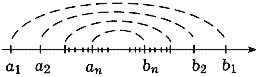
\includegraphics[scale=1]{8.jpg}
\end{center}
\textbf{ТЕОРЕМА}. Система вложенных отрезков имеет непустое пересечение.
\newline
\newline
\textbf{Доказательство}:
\newline
\newline
Пусть задана система вложенных отрезков 
$$ [\,a_{1},b_{1}\,],\,[\,a_{2},b_{2}\,],\ldots,[\,a_{n},b_{n}\,],\ldots;\, a_{n},b_{n}\in\R,\,n=1,2,\ldots.  $$
Обозначим через $A$ множество всех левых концов $a_{n}$ отрезков этой системы, а через $B$ -- множество их правых концов $b_{n}$. Из неравенства
$$ a_{1}\leqslant a_{2}\leqslant\ldots\leqslant a_{n}\leqslant b_{n}\leqslant\ldots\leqslant b_{2}\leqslant b_{1} $$
следует, что 
$$ \forall m,n\in\R:a_{m}\leqslant b_{n}. $$
Поэтому по свойству непрерывности действительных чисел существует такое число $\xi$, что для всех номеров $m$ и $n$ выполняется неравенство $a_{m}<\xi<b_{n}, $ а в частности, неравенство $$a_{n}\leqslant\xi\leqslant b_{n},\,n=1,2,\ldots$$
Это и означает, что точка $\xi$ принадлежит всем отрезкам $ [\,a_{n},b_{n}\,] $.

\newpage
\section{БИЛЕТ 16 -- Теорема о существовании верхней и нижней граней}
\textbf{Верхняя грань множества} -- наименьшее число из множества верхних границ множества.
$$ \exists\: M\in\R\:\forall a\in A:a\leqslant M\quad(\forall m\geqslant M) $$
Множество чисел $m$ -- верхние границы множества $A$, число $M$ -- верхняя грань множества $A$, само множество $A$ называется \textit{ограниченным сверху}. Иными словами, $M$ это \textit{супремум} $A$ $\Rightarrow\:M=sup\,A$.
\newline
\newline
\textbf{Нижняя грань множества} -- наибольшее число из множества нижних границ множества.
$$ \exists\: M\in\R\:\forall a\in A:a\geqslant M\quad(\forall m\leqslant M) $$
Множество чисел $m$ -- нижние границы множества $A$, число $M$ - нижняя грань множества $A$, само множество $A$ называется \textit{ограниченным снизу}. Иными словами, $M$ это \textit{инфимум} $A$ $\Rightarrow\:M=inf\,A$.
\newline
\newline
\textbf{ТЕОРЕМА О СУЩЕСТВОВАНИИ ВЕРХНЕЙ И НИЖНЕЙ ГРАНЕЙ}
\newline
Если $X\ne\varnothing$ и $X$ ограничено сверху (снизу), то 
$$ \exists\:\sup\,X<\infty\quad (\exists\:\inf\,X>-\infty) $$
\textbf{Доказательство} (для верхней грани, для нижней аналогично):
\newline
\newline
Пусть $M$ -- множество всех верхних границ множества $X$, то есть $X\leqslant M$.Тогда
$$ \exists \:c\in\R:X\leqslant c\leqslant M $$
\begin{equation}\label{1}
\setcounter{equation}{1}
    X\leqslant c\leqslant M\:\Rightarrow\:X\leqslant c;
\end{equation}
\begin{equation}\label{2}
    X\leqslant c\leqslant M\:\Rightarrow\: c\leqslant E;
\end{equation}
Исходя из условий (1) и (2),
$$ c=sup\,X<\infty $$
\newpage
\section{БИЛЕТ 17 -- Теорема о пределе монотонной последовательности}
Если последовательность $\{x_{n}\}$  является нестрого возрастающей (нестрого убывающей) и ограничена сверху (снизу), то $\{x_{n}\}$ является сходящейся, причем для неубывающей:
$$ \lim_{n\to\infty} x_{n}=sup\,x_{n}, $$
а для невозрастающей:
$$ \lim_{n\to\infty} x_{n}=inf\,x_{n}. $$
Иными словами, любая монотонная и ограниченная последовательность $\{x_{n}\}$  имеет предел.
\newline
\newline
\textbf{Доказательство}:
\newline
\newline
Пусть последовательность $x_{n}$ является неубывающей ограниченной последовательностью.
Поскольку последовательность неубывающая, то для всех $n$ выполняются неравенства $x_{n+1}\geqslant x_{n}$.\newline
\newline
Поскольку последовательность ограничена, то она имеет точную верхнюю границу $a=sup\,x_{n}$. Это означает, что:

\begin{equation}
\setcounter{equation}{1}
\qquad\forall n: x_{n}\leqslant a;
\end{equation}
\begin{equation}
\forall \xi>0\:\:\exists\: N=N(\xi):x_{N}>a-\xi
\end{equation}
Поскольку последовательность $\{x_{n}\}$ неубывающая, то при $n>N$ имеем 
\begin{equation}
    x_{n}\geqslant x_{N}>a-\xi
\end{equation}
Здесь мы также использовали (2). Комбинируя с (1), находим: $ a-\xi<x_{n}\leqslant a $ при $n>N.$
\newline
Поскольку $a<a+\xi$, то $a-\xi<x_{n}<a+\xi,$ или
$$ |x_{n}-a|<\xi\:\forall n>N. $$
Это и означает, что число $a=sup\,x_{n}$ является пределом последовательности $\{x_{n}\}$.

\newpage
\section{БИЛЕТ 18 -- Определение числа $e$, соответствующий замечательный предел}
$e$ — основание натурального логарифма, математическая константа, иррациональное число. Иногда число $e$ называют числом Эйлера или числом Непера.
\newline
\newline
\textbf{ВТОРОЙ ЗАМЕЧАТЛЬНЫЙ ПРЕДЕЛ}
$$\bigg(1+\frac{1}{n}\bigg)^{n}\to e  $$
\textbf{СЛЕДСТВИЕ ИЗ ФОРМУЛЫ МУАВРА-СТИРЛИНГА}
$$ \lim_{n\to\infty}\frac{n}{\sqrt[n]{n!}}=e $$
\newpage
\section{БИЛЕТ 19 -- Свойства верхнего и нижнего пределов}
Предел, конечный или определенного знака
бесконечный, подпоследовательности данной
последовательности называется ее \textbf{частичным пределом}.
\newline
\newline
Всякая последовательность имеет хотя бы один
частичный конечный или бесконечный предел, причем
заведомо конечный, если данная последовательность
ограничена.
\newline
\newline
Наибольший частичный предел последовательности
называется ее \textbf{верхним пределом}, наименьший частичный предел -- \textbf{нижним пределом}.
$$ \underset{n\to\infty}{\overline{\text{lim} }}x_{n}=M_{1}\qquad \underset{n\to\infty}{\underline{\text{lim} }}x_{n}=M_{2} $$
\newline
У любой последовательности существует как наибольший, так и наименьший частичный предел.
\newline
\newline
\textbf{СВОЙСТВА}
\begin{enumerate}
    \item Существует подпоследовательность $\{x_{n_{k}}\}$ последовательности $\{x_{n}\}$, сходящаяся к верхнему пределу $M_{1}$.
    $$ \lim_{k\to\infty}x_{n_{k}}=M_{1}$$
    \item Для любой сходящейся подпоследователньости $\{x_{n_{k}}\}$ последовательности $\{x_{n}\}$:
    $$ \lim_{k\to\infty}x_{n_{k}}\leqslant M_{1} $$
\end{enumerate}
$$ $$
\begin{enumerate}
    \item Существует подпоследовательность $\{x_{n_{k}}\}$ последовательности $\{x_{n}\}$, сходящаяся к нижнему пределу $M_{2}$.
    $$ \lim_{k\to\infty}x_{n_{k}}=M_{2}  $$
    \item Для любой сходящейся подпоследователньости $\{x_{n_{k}}\}$ последовательности $\{x_{n}\}$:
    $$ \lim_{k\to\infty}x_{n_{k}}\geqslant M_{2} $$
\end{enumerate}
\newpage
\section{БИЛЕТ 20 -- Ряд. Необходимое условие сходимости ряда}
Пара последовательностей $\{u_{n}\}$ и $\{s_{n}\},\;u_{n},\,s_{n}\in\R,\;n=1,2,\ldots$, где $$ s_{n}=u_{1}+u_{2}+\ldots+u_{n}, $$
называется \textbf{рядом}, или \textbf{бесконечной суммой}, и обозначается как
$$ u_{1}+u_{2}+\ldots+u_{n}+\ldots=\sum_{n=1}^{\infty}u_{n} $$
Элементы последовательности $\{u_{n}\}$ называются \textit{членами ряда}, а элементы последовательности $\{s_{n}\}$ -- его \textit{частичными суммами}.
\newline
Если существует конечный предел 
$$ \lim_{n\to\infty}s_{n}=s, $$
то он называется \textit{суммой ряда} и ряд называется \textit{сходящимся}, в ином случае -- \textit{расходящимся}.
\newline
\newline
\textbf{НЕОБХОДИМОЕ УСЛОВИЕ СХОДИМОСТИ РЯДА.}
Если ряд сходится, то последовательность всех его членов стремится к нулю.
\newline
\newline
\textbf{Доказательство}:
\newline
\newline
Если ряд сходится, то есть существует конечный предел последовательности его частичных сумм $s_{n}$, то из равенства $u_{n}=s_{n}-s_{n-1},\,n=1,2,\ldots$ следует, что
$$ \lim_{n\to\infty}u_{n}=\lim_{n\to\infty}s_{n}-\lim_{n\to\infty}s_{n-1}=s-s=0. $$
\textbf{ЛИНЕЙНАЯ КОМБИНАЦИЯ СХОДЯЩИХСЯ РЯДОВ СХОДИТСЯ.}

\newpage
\section{БИЛЕТ 21 -- Критерий Коши сходимости ряда}
Для того чтобы ряд сходился, необходимо и достаточно, чтобы
$$ \forall\xi>0\:\:\exists\:n_{0}\:\forall n>n_{0},\:\forall p\geqslant0:|u_{n}+u_{n+1}+\ldots+u_{n+p}|<\xi $$
\textbf{Доказательство}:
\newline
\newline
Равенство следует непосредственно из критерия Коши для существования конечного предела последовательности, примененного к последовательности частичных сумм радяа, так как
$$ u_{n}+u_{n+1}+\ldots+u_{n+p}=s_{n+p}-s_{n-1}. $$
P.S.: при $p=0$ получаем еще одно доказательство необходимого условия сходимости ряда.
\newpage
\section{БИЛЕТ 22 -- Признак Даламбера}
Пусть для ряда 
$$ \sum_{n=1}^{\infty}u_{n},\,u_{n}>0,\,n=1,2,\ldots $$
существует предел
$$ \lim_{n\to\infty}\frac{u_{n+1}}{u_{n}}=l. $$
Тогда если $l<1$, то ряд сходится, а если $l>1$ --  расходится.
\newline
\newline
Если $l=1$, то ничего определенного сказать нельзя (теорема не подходит).
\newline
\newline
\textbf{Доказательство}:
\newline
\newline
Пусть $l<1.$ Выберем число $q$ так, чтобы $l<q<1.$
$$ \lim_{n\to\infty}\frac{u_{n+1}}{u_{n}}=l \:\Rightarrow$$
$$\Rightarrow\:\:\exists\:n_{0}>1\:\forall n>n_{0}:\frac{u_{n+1}}{u_{n}}<q\:\Rightarrow\:u_{n+1}<u_{n}\cdot q$$
Применяя конечное неравенство последовательно, получим
$$ u_{n_{0}+1}<u_{n_{0}}\cdot q^{1};\; u_{n_{0}+2}<u_{n_{0}+1}\cdot q^{2};\;\ldots;\; u_{n_{0}+k}<u_{n_{0}+k-1}\cdot q^{k}$$
Ряд $u_{n_{0}}\cdot\sum_{k=1}^{\infty}q^{k}$ в силу условия $0<q<1$ сходится, поэтому по признаку сравнения сходится ряд $\sum_{k=1}^{\infty}u_{n_{0}+k}.$ Следовательно, сходится и ряд $\sum_{k=1}^{\infty}u_{k}.$
\newline
\newline
\newline
Пусть теперь $l>1.$
$$ \lim_{n\to\infty}\frac{u_{n+1}}{u_{n}}=l \:\Rightarrow$$
$$\Rightarrow\:\:\exists\:n_{0}>1\:\forall n>n_{0}:\frac{u_{n+1}}{u_{n}}>1\:\Rightarrow\:u_{n+1}>u_{n}.$$
Применяя последовательно для больших номеров $n_{0},$ получим
$$ u_{n+1}>u_{n}>\ldots>u_{n_{0}+1}>n_{0}>0.$$
Последовательность членов ряда не стремится к нулю, а значит ряд $\sum_{n=1}^{\infty}u_{n}$ расходится.
\newpage
\section{БИЛЕТ 23 -- Признак Коши (радикальный)}
Пусть для ряда 
$$ \sum_{n=1}^{\infty}u_{n},\,u_{n}>0,\,n=1,2,\ldots $$
существует предел
$$ \lim_{n\to\infty}\sqrt[n]{u_{n}}=l. $$
Тогда если $l<1$, то ряд сходится, а если $l>1$ -- расходится.
\newline
\newline
Если $l=1$, то ничего определенного сказать нельзя (теорема не подходит).
\newline
\newline
\textbf{Доказательство}:
\newline
\newline
Пусть $l<1$. Выберем число $q$ так, чтобы $l<q<1.$
$$ \lim_{n\to\infty}\sqrt[n]{u_{n}}=l \:\Rightarrow $$
$$ \Rightarrow\:\exists\:n_{0}\:\forall n>n_{0}:u_{n}<q^{n}.$$
Так как ряд $\sum_{n=0}^{\infty}q^{n}$ сходится, то сходится и ряд $\sum_{k=1}^{\infty}u_{n_{0}+k}.$ Это означает сходимость ряда $\sum_{n=1}^{\infty} u_{n}.$
\newline
\newline
Пусть теперь $l>1.$
$$ \lim_{n\to\infty}\sqrt[n]{u_{n}}=l \:\Rightarrow $$
$$ \Rightarrow\:\exists\:n_{0}\:\forall n>n_{0}: \sqrt[n]{u_{n}}>1\:\Rightarrow\:u_{n}>1.$$
Следовательно, последовательность членов ряда не стремится к нулю, значит ряд $\sum_{n=1}^{\infty} u_{n}$ расходится.
\newpage
\section{БИЛЕТ 24 -- Признак сравнения}
Пусть $0\leqslant u_{n}\leqslant v_{n}$. Тогда:
\begin{itemize}
    \item Если ряд $ \sum_{n=1}^{\infty}v_{n} $ сходится, то сходится и ряд $ \sum_{n=1}^{\infty}u_{n} $.
    \item Если ряд $ \sum_{n=1}^{\infty}u_{n} $ расходится, то расходится и ряд $ \sum_{n=1}^{\infty}v_{n} $.
\end{itemize}
\textbf{Доказательство}:
\newline
\newline
Если ряд $ \sum_{n=1}^{\infty}v_{n} $
сходится, то есть имеет конечную сумму 
$$ \sigma=\sum_{n=1}^{\infty} v_{n},\; \sigma_{n}=\sum_{k=1}^{n} v_{n_{k}},\: \forall n=1,2,\ldots :\sigma_{n}<\sigma.$$
$$ 0\leqslant u_{n}\leqslant v_{n}\:\Rightarrow $$
$$ \Rightarrow\:s_{n}\leqslant \sum_{k=1}^{n} u_{k}\leqslant\sum_{k=1}^{n} v_{k}=\sigma_{n}\leqslant\sigma,$$
А это (в силу леммы*) означает, что ряд ($u_{1}+u_{2}+\ldots+u_{n}+\ldots$) сходится.
\newline
\newline
Если ряд $ \sum_{n=1}^{\infty}u_{n} $ расходится, то ряд $ \sum_{n=1}^{\infty}v_{n} $ тоже расходится, иначе бы сходился ряд $ \sum_{n=1}^{\infty}u_{n} $ по доказанному выше.
\newline
\newline
*\textit{Лемма}. Если члены ряда неотрицательны, то он сходится тогда и только тогда, когда его частичные суммы ограничены сверху.
\newline
\newline
\textbf{СЛЕДСТВИЯ}
\newline
\newline
Пусть $u_{n}\geqslant0,\,v_{n}>0,\,n=1,2,\ldots$ и
$$ \lim_{n\to\infty}\frac{u_{n}}{v_{n}}=l, $$
тогда:
\begin{itemize}
    \item Если ряд $ \sum_{n=1}^{\infty}v_{n} $ сходится и $0\leqslant l<+\infty$, то сходится и ряд $ \sum_{n=1}^{\infty}u_{n} $
    \item Если ряд $ \sum_{n=1}^{\infty}v_{n} $ расходится и $0<l\leqslant+\infty$, то расходится и ряд $ \sum_{n=1}^{\infty}u_{n} $
\end{itemize}
\newpage
\section{БИЛЕТ 25 -- Абсолютная и условная сходимость знакопеременных рядов}
\begin{center}
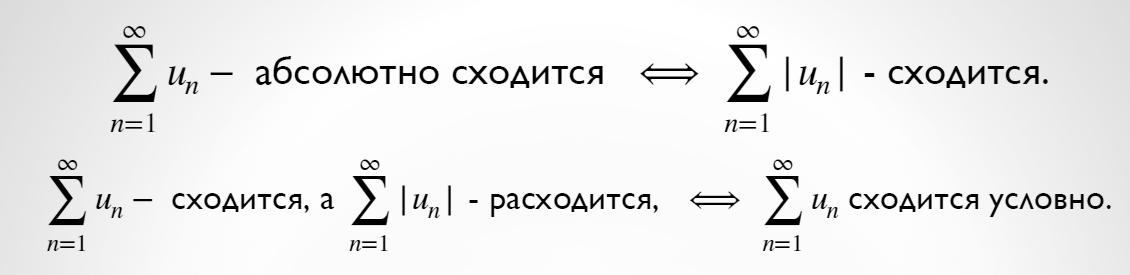
\includegraphics[scale=0.4]{7.jpg}
\end{center}
\textbf{ТЕОРЕМА 1}.Абсолютно сходящийся ряд сходится.
\newline
\newline
\textbf{Доказательство}:
$$ \sum_{i=0}^{n}|u_{n}|=S\in\R\:\Rightarrow $$
$$\Rightarrow\:\exists\:n_{0}\,(\forall n>n_{0}\,\land\,\forall p\in\Z):\sum_{k=0}^{p}|u_{n+k}|<\xi.  $$
$$ \left| \sum_{k=0}^{p} u_{n+k} \right|\leqslant\sum_{k=0}^{p}|u_{n+k}|<\xi\:\Rightarrow\:\sum_{i=0}^{n}u_{n}=S\in\R. $$
\textbf{ТЕОРЕМА 2}. Линейная комбинация абсолютно сходящихся рядов есть абсолютно сходящийся ряд.
\newline
\newline
\textbf{Доказательство}:
$$ \sum_{n=1}^{\infty}|u_{n}|=U\in\R,\,\sum_{n=1}^{\infty}|v_{n}|=V\in\R\:\Rightarrow $$
$$ \forall\lambda,\mu\in\R:\:\sum_{n=1}^{\infty}|\lambda|\cdot|u_{n}|+|\mu|\cdot|v_{n}|=\lambda\cdot U+\mu\cdot V\in\R $$
$$|\lambda\cdot u_{n}+\mu\cdot v_{n}|\leqslant|\lambda|\cdot |u_{n}|+|\mu|\cdot |v_{n}|\:\Rightarrow$$
$$ \Rightarrow\:\sum_{n=1}^{\infty}|\lambda\cdot u_{n}+\mu\cdot v_{n}|=S\in\R\:\Rightarrow $$
$$\sum_{n=1}^{\infty}\lambda\cdot u_{n}+\mu\cdot v_{n}=\Sigma\in\R.  $$
\newpage
\textbf{ТЕОРЕМА 3}. Если ряд абсолютно сходится, то любой ряд, составленный из членов данного ряда, но взятых в другом порядке, также абсолютно сходится и имеет ту же сумму.
$$ \sum_{n=1}^{\infty}|u_{n}|=U\in\R\:\Rightarrow $$
$$ \Rightarrow\:\forall \{u_{n_{k}}\}:\sum_{k=1}^{\infty}u_{n_{k}}=\Sigma\in\R,\,\sum_{n=1}^{\infty}u_{n}=\sum_{k=1}^{\infty}u_{n_{k}}=U. $$
\textbf{ТЕОРЕМА 4}. Если ряды абсолютно сходятся, то ряд, составленный из всевозможных попарных произведений членов этих рядов, также абсолютно сходится, причем его сумма равна произведению сумм этих рядов.
$$ \sum_{m=1}^{\infty}|u_{m}|=U\in\R,\,\sum_{n=1}^{\infty}|v_{n}|=V\in\R,$$
$$ \sum u_{m}\cdot v_{n}=U\cdot V. $$
\textbf{Доказательство}:
$$ u_{1}\cdot v_{1}\quad u_{1}\cdot v_{2}\quad\ldots\quad u_{1}\cdot v_{n}\quad\ldots $$
$$ u_{2}\cdot v_{1}\quad u_{2}\cdot v_{2}\quad\ldots\quad u_{2}\cdot v_{n}\quad\ldots $$
$$\ldots\ldots\ldots\ldots\ldots\ldots\ldots\ldots\ldots\ldots\ldots\ldots$$
$$ u_{m}\cdot v_{1}\quad u_{m}\cdot v_{2}\quad\ldots\quad u_{m}\cdot v_{n}\quad\ldots $$
$$\ldots\ldots\ldots\ldots\ldots\ldots\ldots\ldots\ldots\ldots\ldots\ldots$$
$$  $$
$$ u_{1}\cdot v_{1}+u_{1}\cdot v_{2}+u_{2}\cdot v_{2}+u_{2}\cdot v_{1}+\ldots $$
$$ |u_{1}\cdot v_{1}|+|u_{1}\cdot v_{2}|+|u_{2}\cdot v_{2}|+|u_{2}\cdot v_{1}|+\ldots $$
$$ \sum_{k=1}^{n}|u_{k}|=U_{n}\in\R,\,\sum_{k=1}^{n}|v_{k}|=V_{k}\in\R,\,s_{n}=\sum_{k=1}^{n}|u_{m_{k}}\cdot v_{n_{k}}|. $$
$$ s_{1}=|u_1\cdot v_1|=U_1\cdot V_1 $$
$$ s_4=|u_{1}\cdot v_{1}|+|u_{1}\cdot v_{2}|+|u_{2}\cdot v_{2}|+|u_{2}\cdot v_{1}|=(|u_1|+|u_2|)\cdotv(|v_1|+|v_2|)=U_2\cdot V_2\leqslant U\cdot V $$
$$\ldots\ldots\ldots\ldots\ldots\ldots\ldots\ldots\ldots\ldots\ldots\ldots$$
$$ s_{n^2}=(|u_1|+|u_2|+\ldots+|u_n|)\cdot(|v_1|+|v_2|+\ldots|v_n|)=U_n\cdot V_n\leqslant U\cdot V. $$
$$\ldots\ldots\ldots\ldots\ldots\ldots\ldots\ldots\ldots\ldots\ldots\ldots$$
$$ \sum_{k=1}^{\infty}u_{m_k}\cdot v_{n_k}=U\cdot V $$

\newpage
\section{БИЛЕТ 26 -- Теорема Лейбница}
Если члены знакочередующегося ряда монотонно убывают по модулю, то ряд сходится.
$$ \lim_{n\to\infty}u_{n}=0,\,u_{n}\geqslant u_{n+1}>0,\,n=1,2,\ldots; $$
$$ \sum_{n=1}^{\infty}(-1)^{n+1}\cdot u_{n}=S\in \R; $$
$$ |S-S_{n}|\leqslant u_{n+1}. $$
\textbf{Доказательство}:
$$ S_{2k}=\sum_{n=1}^{2k}(-1)^{n+1}\cdot u_n=(u_1-u_2)+(u_3-u_4)+\ldots+(u_{2k-1}-u_{2k}). $$
$$ u_{2k-1}-u_{2k}\geqslant0\:\Rightarrow\:S_{2k}\leqslant S_{2k+2} $$
$$S_{2k}=u_1-(u_2-u_3)-\ldots-(u_{2k-2}-u_{2k-1})-u_{2k}\:\Rightarrow\:S_{2k}<u_1\:\Rightarrow $$
$$ \Rightarrow\:\lim_{k\to\infty}S_{2k}=S. $$
$$ S_{2k+1}=S_{2k}+u_{2k+1}=\Bigg(\sum_{n=1}^{2k}(-1)^{n+1}\cdot u_n\Bigg) +u_{2k+1}.$$
$$ \lim_{k\to\infty} u_{2k+1}=0\:\Rightarrow\:\lim_{k\to\infty}S_{2k+1}=S;\;\lim_{k\to\infty} S_n=S.\:\Rightarrow $$
$$ S_{2k+1}=S_{2k-1}-(u_{2k}-u_{2k+1})\leqslant S_{2k-1}\:\Rightarrow\:S\leqslant S_{2k-1}. $$
$$  $$
\begin{equation}
    \setcounter{equation}{1}
    S-S_{2k}\leqslant S_{2k+1}-S_{2k}=u_{2k+1};
\end{equation}
\begin{equation}
    S_{2k-1}-S\leqslant S_{2k-1}-S_{2k}=u_{2k}.
\end{equation}
По индукции [условия (1) и (2)] доказано, что
$$ |S-S_n|\leqslant u_{n+1}. $$
\newpage
\section{БИЛЕТ 27 -- Теорема Римана}
Если ряд сходится условно и если $A$ – любое число или любой из символов бесконечности, то надлежаще выбранной перестановкой членов этого ряда можно всегда заставить новый ряд сходиться к $A$.
\newline
\newline
\textbf{Доказательство}:
$$ \sum_{m=1}^{\infty}u_{m}^{+}=+\infty,\;\sum_{k=1}^{\infty}u_{k}^{-}=+\infty $$
$$ u_{1}^{+}+u_{2}^{+}+\ldots+u_{n_{1}}^{+}>A; $$
$$ u_{1}^{+}+u_{2}^{+}+\ldots+u_{n_{1}-1}^{+}\leqslant A; $$
$$ u_{1}^{+}+u_{1}^{+}+\ldots+u_{n_{1}}^{+}-u_{1}^{-}-u_{2}^{-}-\ldots-u_{n_{2}}^{-}<A; $$
$$ u_{1}^{+}+u_{2}^{+}+\ldots+u_{n_{1}}^{+}-u_{1}^{-}-u_{2}^{-}-\ldots-u_{n_{2}-1}^{-}\geqslant A. $$
$$  $$
$$ u_{1}^{+}+u_{2}^{+}+\ldots+u_{n_{1}}^{+}-u_{1}^{-}-u_{2}^{-}-\ldots-u_{n_{2}}^{-}+u_{n_{2}+1}+\ldots+u_{n_{3}}^{+}-u_{n_{2}+1}^{-}-\ldots-u_{n_{4}}^{-}+u_{n_{3}+1}^{+}+\ldots $$
$$ s_{n_{1}},\,s_{n_{1}+n_{2}},\,s_{n_{2}+n_{3}},\ldots,\,s_{n_{k}+n+{k+1}},\,\ldots $$
$$ s_{n_{1}}>A,\,s_{n_{1}+n_{2}}<A,\,s_{n_{2}+n_{3}}>A,\ldots $$
$$ |A-s_{n_{k}+n_{k+1}}|\leqslant u_{n_{k+1}}^{\pm}<\xi\:\Rightarrow\:\lim_{k\to\infty}s_{n_{k}+n_{k+1}}=A. $$
$$ n>n_{1}+n_{2},\; \exists\:k: $$
$$ (s_{n_{k}+n_{k+1}}\leqslant s\leqslant s_{n_{k+1}+n_{k+2}}) \land (s_{n_{k}+n_{k+1}}\geqslant s\geqslant s_{n_{k+1}+n_{k+2}}) \:\Rightarrow $$
$$\Rightarrow\:\lim_{n\to\infty} s_{n}=A$$







\end{document}